\documentclass[a4paper]{report}

\usepackage[utf8]{inputenc}
\usepackage[english]{babel}
\usepackage[T1]{fontenc}
\usepackage{textcomp}
\usepackage[]{amsthm} 
\usepackage[]{amssymb}
\usepackage{graphicx}
\usepackage{float}
\usepackage{soul}
\usepackage{color}
\usepackage{bm}
\usepackage{listings}
\usepackage{xcolor}
\usepackage{enumitem}
%\usepackage{xfrac}
\usepackage[normalem]{ulem}

% ~~~~ no indent per paragraph ~~~~-
\usepackage[parfill]{parskip}

% ~~~~ hyperlinks ~~~~ 
\usepackage[colorlinks=true, linkcolor=blue]{hyperref}

% ~~~~ subfigs ~~~~
\usepackage{subcaption}

% ~~~~ math ~~~~
\usepackage{amsmath}

\usepackage{mathtools}
% ~~ colorbox : "align" use only ~~
\newcommand{\myboxA}[1]{
	\fcolorbox{black}{lime}{#1}
}
\MakeAboxedCommand\AboxedA\myboxA

% ~~ colorbox : else ~~
\newcommand{\mybox}[1]{
	\fcolorbox{black}{lime}{$\displaystyle#1$}
}

% ~~~~ graphics ~~~~
\usepackage{tikz}
\usetikzlibrary{trees}
\usetikzlibrary {fit,shapes.geometric} % W: Command terminated with space. (1)
\usetikzlibrary {automata} % W: Command terminated with space. (1)
\usetikzlibrary{arrows.meta}
\usepackage{multicol}

\usepackage{pgfplots}
\pgfplotsset{compat = newest}

\usepackage{geometry}
\geometry{legalpaper, margin=1in}

% ~~~~ upgraded tables ~~~~
\usepackage{booktabs}

% ~~~~ algorithm formatting ~~~~
\usepackage{algorithm}
\usepackage[noend]{algpseudocode}
\usepackage{caption}

% ~~~~ list bullets ~~~~
\renewcommand{\labelitemii}{$\circ$}
\renewcommand{\labelitemiii}{$\star$}
\renewcommand{\labelitemiv}{$>$}

% figure support
\usepackage{import}
\usepackage{xifthen}
\pdfminorversion=7
\usepackage{pdfpages}
\usepackage{transparent}
\newcommand{\incfig}[1]{%
    \def\svgwidth{\columnwidth}
    \import{./figures/}{#1.pdf_tex}}

% Newline for algorithm psuedo
\newcommand{\algrule}[1][.2pt]{\par\vskip.5\baselineskip\hrule height #1\par\vskip.5\baselineskip}

% -------- Listings/XColor Settings --------
\definecolor{codegreen}{rgb}{0,0.6,0}
\definecolor{codegray}{rgb}{0.5,0.5,0.5}
\definecolor{codepurple}{rgb}{0.58,0,0.82}
\definecolor{backcolour}{rgb}{0.95,0.95,0.92}

\lstdefinestyle{mystyle}{
	backgroundcolor=\color{backcolour},
	commentstyle=\color{codegreen},
	keywordstyle=\color{magenta},
	numberstyle=\tiny\color{codegray},
	stringstyle=\color{codepurple},
	basicstyle=\ttfamily\scriptsize,
	breakatwhitespace=false,
	breaklines=true,
	captionpos=b,
	keepspaces=true,
	numbers=left,
	numbersep=5pt,
	showspaces=false,
	showstringspaces=false,
	showtabs=false,
	tabsize=4
}

\lstset{style=mystyle}

% -------------- Doc Start -------------------



\pdfsuppresswarningpagegroup=1

\title{\Huge{Naive RISCV-I Pipeline}}
\author{\textbf{Authors:} WhisperingRock\\}
\date{CPE333\\ \small{Fall2026} \\ \today}

\begin{document}
    \maketitle

	% ~~~~ add toc as a bookmark ~~~~
	\phantomsection
	\addcontentsline{toc}{section}{\contentsname}

	\tableofcontents

	\chapter{Introduction}
		In this report, an implementation of a naive RISCV-I Otter is constructed
		and tested against a simple piece of assembly. This design is 
		considered naive because we must manually include \texttt{nop} in our 
		assembly code to mitigate data hazards. 

	\chapter{Design}
	
		To convert our multicycle otter to a pipelined one, pipe registers
		are needed and stages be implemented. 

		The stages are 
		\begin{itemize}
			\item \textbf{IF} : The PC \textbf{I}nstruction \textbf{F}etched from ram/memory.
			\item \textbf{DE} : The instruction \textbf{DE}coded and register values gathered.
			\item \textbf{EX} : The instruction is \textbf{EX}ecuted and result stored / branch prep.
			\item \textbf{MEM}: A directed read or write to \textbf{MEM}ory occurs. 
			\item \textbf{WB} : \textbf{W}rite results \textbf{B}ack to register.
		\end{itemize}

		\begin{figure}[H]
			\centering
			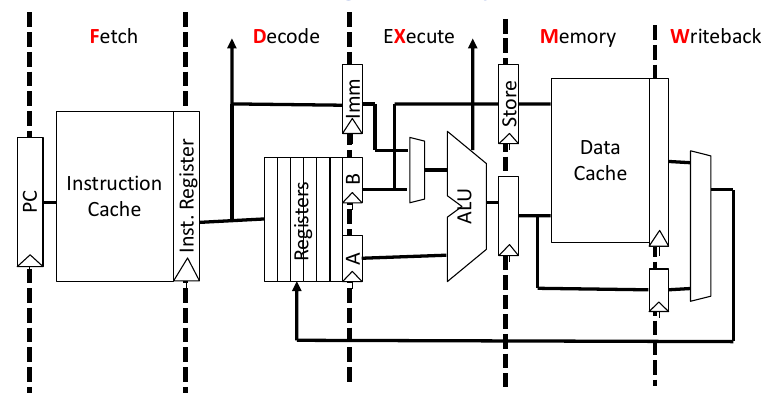
\includegraphics[
				width			= 0.5\textwidth,
				keepaspectratio	= true
			]{../simple_pipe.png}
			\caption{Example of Naive RISCV-I Pipeline}
			\label{fig:simple-pipe}
		\end{figure}

		\begin{figure}[H]
			\centering
			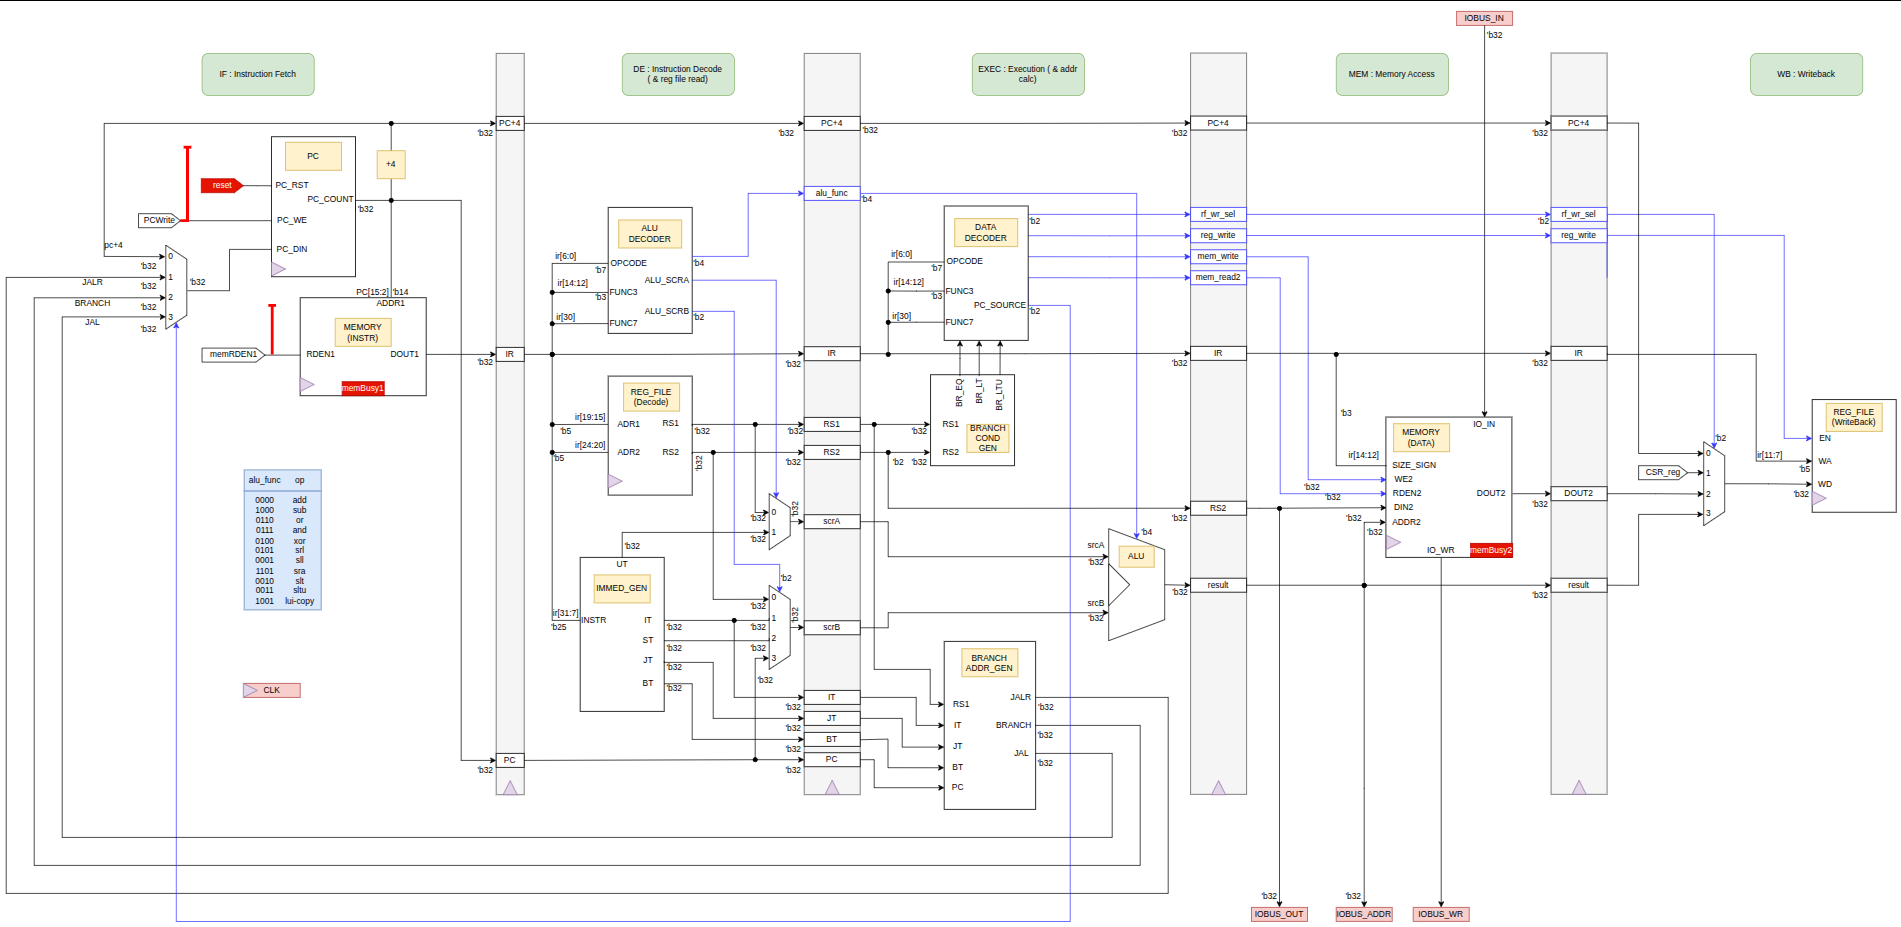
\includegraphics[
				width			= 1\textwidth,
				keepaspectratio	= true,
			]{../pipeline_nohaz.png}
			\caption{Detailed Naive RISCV-I Pipeline}
			\label{fig:detail-pipe}
		\end{figure}

		Modules updated to implement the pipeline (from CPE's 233 Multicycle Otter):
		\begin{itemize}
			\item Remove CSR components
			\item \textbf{MCU} received re-org and pipe registers \ref{otter:mcu-pipe}.
			\item \textbf{RegFile} changed to write on negative edge \ref{otter:rf} 
				in order to perform writes in \textbf{WB} and reads in \textbf{DE}.
			\item The Control Unit FSM was removed because it is made redundant 
				with the pipeline
			\item The Control Unit Decoder was split into two parts, \ref{otter:alu-dc} 
				and \ref{otter:data-dc}, to shorting propagation timing. 
		\end{itemize}
		
	\chapter{Testing}

		A simple test program was given to ensure our restructure was 
		surface-level correct enough to be able to handle WB writes and 
		DE reads of the same variable. Due to the default memory mapping 
		below, an additional instruction was used to load the lengthy 
		DATA segment address along with the appropriate number of \texttt{nop}s.

		\begin{figure}[H]
			\centering
			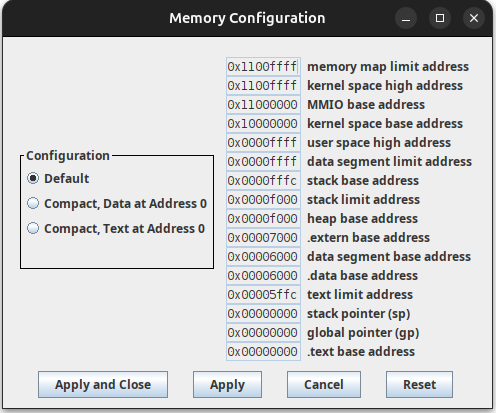
\includegraphics[
				width			= 0.6\textwidth,
				keepaspectratio	= true
			]{../setting_memmap.png}
			\caption{Memory Mapping}
			\label{fig:memmap}
		\end{figure}	

		\lstinputlisting[
			language 	= {[riscv]Assembler},
			captionpos	= top, 
			caption		= {\texttt{l3test\_given\_updated.sv}},
			breaklines	= false, 
			label		= {otter:pipe-test}
		]{../given/l3test_given_updated.asm}

		\begin{figure}[H]
			\centering
			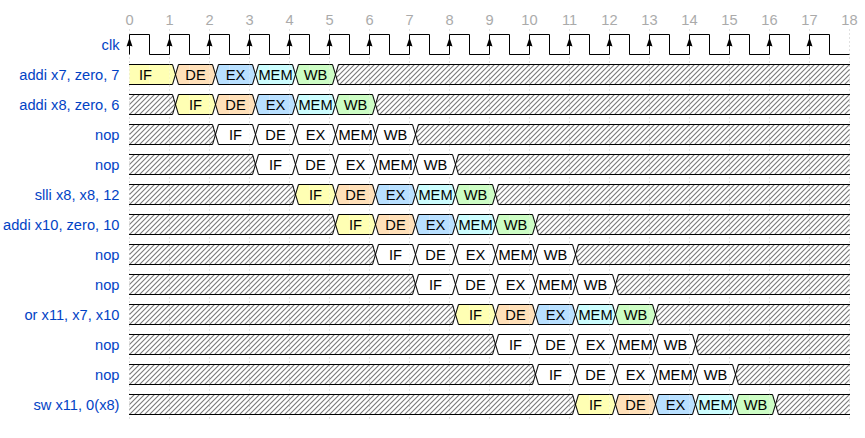
\includegraphics[
				width			= \textwidth,
				keepaspectratio	= true
			]{../updated_timing.png}
			\caption{Expected Timing Nearing 15 Cycles}
			\label{fig:test-timing}
		\end{figure}

	\chapter{Results}
	
		\begin{figure}[H]
			\centering
			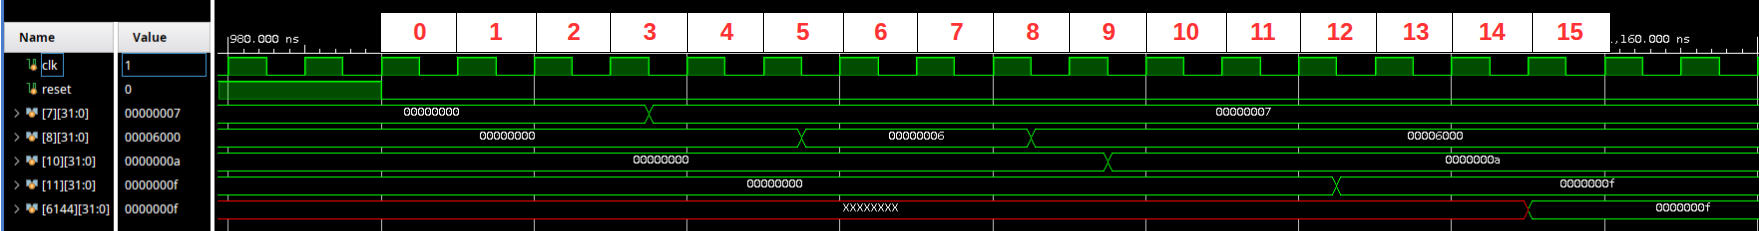
\includegraphics[
				width			= \textwidth,
				keepaspectratio	= true
			]{../sim_result.png}
			\caption{Simulation Results}
			\label{fig:sim-result}
		\end{figure}

		Timings above are on par with the expected result in \ref{fig:test-timing} such that
		we take 15 cycles to load \texttt{0xF} into the address and each cycle reaches
		their respective WB or MEM in cadence with \ref{fig:test-timing}.


		Moreover, an explanation is owed as to why there is a difference between
		our input address of \texttt{0x6000} in \ref{otter:pipe-test} 
		and the output location of \texttt{mem[6144]} in \ref{fig:sim-result}.
		Consider that the memory blocks are in increments of bytes, and a block 
		containing 4 of them to make 32 bits, therefore each decimal increase 
		of our simulation memory location goes up by four. Put another way, 
		our DATA segment will be stored at $\frac{32'h0000\_6000}{4} = 32'h0000\_1800 = 32'd6144$.

	\chapter{Conclusion}

		The naive pipeline can perform a select few instructions but we
		the authors must depend on manual placement of \texttt{nop}s until
		we have a solution to deal with hazards.

	\chapter{Appendix}
		\section{Code}

			\lstinputlisting[
				language 	= {verilog},
				captionpos	= top, 
				caption		= {\texttt{Otter\_MCU\_piped.sv}},
				breaklines	= false, 
				label		= {otter:mcu-pipe}
			]{../../../04_hardware/src/Otter_MCU_piped.sv}

			\lstinputlisting[
				language 	= {verilog},
				captionpos	= top, 
				caption		= {\texttt{RegFile.sv}},
				breaklines	= false, 
				label		= {otter:rf}
			]{../../../04_hardware/src/RegFile.sv}

			\lstinputlisting[
				language 	= {verilog},
				captionpos	= top, 
				caption		= {\texttt{Data\_Decoder.sv}},
				breaklines	= false, 
				label		= {otter:data-dc}
			]{../../../04_hardware/src/Data_Decoder.sv}

			\lstinputlisting[
				language 	= {verilog},
				captionpos	= top, 
				caption		= {\texttt{ALU\_Decoder.sv}},
				breaklines	= false, 
				label		= {otter:alu-dc}
			]{../../../04_hardware/src/ALU_Decoder.sv}

\end{document}
